\mode<presentation>
{
  \usetheme{CambridgeUS}
  \usecolortheme{whale}
  \usecolortheme{lily}

  \setbeamercovered{transparent}
  \usefonttheme[onlymath]{serif}
}

\title[\BodeControlDesignIIShortName] % (optional, use only with long paper titles)
{\course: \BodeControlDesignIIName\license}

\subtitle
{Lecture \BodeControlDesignIINumber} % (optional)



\begin{document}

\begin{frame}
  \titlepage
\end{frame}

\mode<article>{
\maketitle
\tableofcontents
}

%\mode<presentation>{
%\begin{frame}{Outline}
%  \tableofcontents
%  % You might wish to add the option [pausesections]
%\end{frame}}
\section{Pre-requisite Material}
This lecture assumes that the reader is familiar with the following material:
\begin{itemize}
	\item Lecture \TimeFrequencyNumber:~\TimeFrequencyName
	\item Lecture \BodeControlDesignINumber:~\BodeControlDesignIName
\end{itemize}

Note: this article makes heavy use of Matlab's ``Control System Designer'' (formerly \texttt{sisotool}) and we recommend that you open that tool and follow along with the article there for full benefit. The two sections use different versions of the tool.

\section{Analysis of PD Control
\label{sec:PDcontrol}}


Let's return to the control design problem from \BodeControlDesignINumber:~\BodeControlDesignIName.

Consider the following system: 
\[
G(s)=\frac{5}{s(s+1)(s+10)}
\]%
We would like to design a controller so that the feedback system has the
following desirable characteristics:

\begin{itemize}
	\item Zero steady state error to a step input
	
	\item Rise time of  1.1 s
	
	\item \% overshoot $\leq 16.5$\%.
\end{itemize}

We found that these time domain specifications gave rise to the following frequency domain specifications:

\begin{itemize}
	\item Loop gain contains an integrator (low frequency gain goes to infinity)
	\item Crossover $\wco=2$ rad/s
	\item Phase margin $\PM = 50^{\circ}$
\end{itemize}

We were unable to meet these specifications using proportional control alone. In particular, we had a very oscillatory response with large \%OS. Let's see if we can make more headway using a PD controller, which adds a zero and can therefore increase the phase margin $\PM$. Recall our PD design block diagram
\begin{frame}{PD Control}
\begin{center}
	\input{figures/PDcontrolloop2.tex}
\end{center}
\end{frame}

In addition to changing the gain at all frequencies by design of $K_{d}$, the PD controller allows us to place a zero in the loop gain via the selection of $K_{p}/K_{d}$.  Let's start the design process by entering the open loop transfer function $G(s)$, loading \texttt{sisotool}, importing $G(s)$, and opening the design plot. A quick way to do this is the following:\vspace{.1in}
\texttt{\\
s = tf([1 0],1);\\
G = 5/(s*(s+1)*(s+10));\\
sisotool(G)\vspace{.1in}\\
}
The design plot figure should look as follows:

\begin{frame}
\begin{center}
\mode<article>{\includegraphics[width=4in]{figures/sisotool1}}
\mode<presentation>{\includegraphics[height=3.4in]{figures/sisotool1}}
\end{center}
\end{frame}

Before, when we increased the gain so that the crossover frequency was $\omega_{co}=2$~rad/s, we ran into problems because the phase margin was poor. We can improve the phase margin by adding a zero near the crossover frequency. Recall from Lecture~\BodePlotsIIINumber:~\BodePlotsIIIName~that the Bode plot for a LHP zero term has a phase that goes from $0^{\circ}$ to $90^{\circ}$ around the zero's break frequency. Remember also that properties of the \texttt{log} and $\angle$ functions mean that Bode plots for different terms can be added together, so by adding this LHP zero we can make the net phase response more positive.

Let's place a zero just before 2 rad/s. To do this, we can click on the zero icon of the design figure circled in green in the figure below. Although we can edit this design in either the root locus or the Bode plot, since this article is about Bode plots we'll use that one. In the Bode plot figure, click on the magnitude plot around 1 rad/s. The result should look like the figure below. If you misplace the zero, you can put the cursor over the zero until it looks like a hand, and the left click to grab the zero and move it right (moving the zero at $s=-\frac{K_p}{K_d}$ to a higher frequency) or left (lower frequency). 

\begin{frame}
\begin{center}
	\mode<article>{\resizebox{4in}{!}{
			\begin{tikzpicture}
			\draw (0,0) node {\includegraphics[width=4in]{figures/sisotool2}};
			\draw (-3.7,4.4) node[circle,very thick=15pt,draw,color=green,inner sep=5pt] (zero) {};
			\draw (2.1,2.6) node (zerobode) {};
			\draw (-6,5) node (click1) {click here};
			\draw (4,3) node (click2) {then click here};
			\draw[->] (click1) -- (zero);
			\draw[->] (click2) -- (zerobode); 
			\end{tikzpicture}}}
	\mode<presentation>{\resizebox{!}{3.4in}{
			\begin{tikzpicture}
			\draw (0,0) node {\includegraphics[width=4in]{figures/sisotool2}};
			\draw (-3.7,4.4) node[circle,very thick=15pt,draw,color=green,inner sep=5pt] (zero) {};
			\draw (2.1,2.6) node (zerobode) {};
			\draw (-6,5) node (click1) {click here};
			\draw (4,3) node (click2) {then click here};
			\draw[->] (click1) -- (zero);
			\draw[->] (click2) -- (zerobode); 
			\end{tikzpicture}}}
\end{center}
\end{frame}

Note that the placement of the zero has changed both the Bode plot and the root locus plot. %The root locus now bends back towards the left, circling the zero. This means that if we now increase the gain, the dominant closed loop poles will also move to the left so that the response is faster, but in addition the damping ratio will be bounded by the angle at the top of the circle. 
For the root locus interpretation, refer back to Lecture~\RootLocusIINumber:~\RootLocusIIName. The phase is higher than for the plant $G(s)$ alone before we added the zero (see Lecture~\BodeControlDesignINumber) because of the control zero we added. 

Next, use the ``hand'' tool (hover over the magnitude Bode plot until it appears) to move the magnitude plot up until the crossover is 2 rad/s. This change of gain is equivalent to increasing the derivative gain $K_d$ in the ``PD Control'' block diagram earlier in this lecture. This action results in the following plot:
\begin{frame}
\begin{center}
\mode<article>{\includegraphics[width=3.7in]{figures/sisotool3}}
\mode<presentation>{\includegraphics[width=3.4in]{figures/sisotool3}}
\end{center}
\end{frame}
Note that the crossover is 2.03 rad/s (as noted in the lower left corner of the phase plot), and the phase margin is $72.4^{\circ}$. These values of $\omega_{co,G}$ and $\PM_{,G}$ meet our specifications from the beginning of this section, so our step response should be acceptable. However, since we have used approximations in the design process (see Lecture~\TimeFrequencyNumber), we always need to verify our design by plotting the step response. 

By clicking on the menu item ``Analysis -> Response to Step Command'' and right clicking on the plots to show the rise time and peak response, we get the following plot:

\begin{frame}
\begin{center}
\mode<article>{\includegraphics[width=4.5in]{figures/sisotool4}}
\mode<presentation>{\includegraphics[width=3.4in]{figures/sisotool4}}
\end{center}
\end{frame}
To recover our controller, we go back to the ``Control and Estimation Tools Manager'',\ and click on ``Compensator Editor.'' \begin{frame}
\begin{center}
\includegraphics[width=4.5in]{figures/sisotool5}
\end{center}
\end{frame}
We see that the controller has the form
\[
C(s) = 5.0299(1+0.78s)
\]
or, multiplying through,
\[
C(s) = 5.0299+ 3.923s
\]
Thus, we should pick $K_{p}=5.0299$ and $K_{d} = 3.923 $

\section{Analysis of PI Control
\label{sec:PIcontrol}}

From our analysis of steady state error, we know that the system type\footnote{Recall that system Type is the number of poles at $s=0$, also called the number of pure integrators} of the loop gain plays a key role. In particular, if zero steady state error for a step input is required, then the system Type must be 1 (or higher). If the plant to be controlled, $G(s)$, does not have a pole at $s=0$, then this must be supplied by the controller. A Proportional-Integral (PI) controller can do this and has the following structure:

\begin{frame}{PI Control}
\begin{center}
	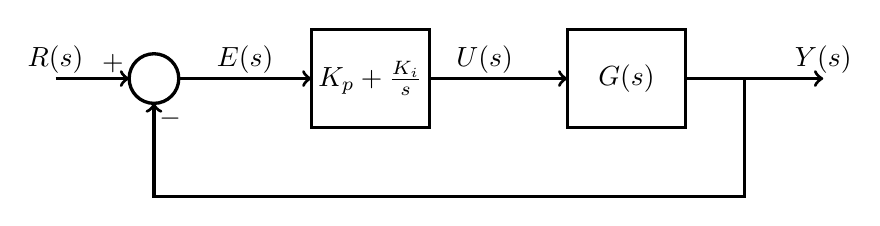
\begin{tikzpicture}[scale=1,inner sep=0pt,outer sep=0pt,very thick,
sysblock/.style={draw,rectangle,inner sep=2pt,minimum width=1.5cm,minimum height=1.25cm,very thick}]

\draw (1.25,0) node[draw,circle] (sum1) {$\rule{0pt}{18pt}$};
\draw (4,0) node[sysblock] (Kp) {$K_{p} + \frac{K_{i}}{s}$};
\draw (7.25,0) node[sysblock] (G) {$G(s)$};

\draw[->] (0,0) node[above=2pt] {$R(s)$} -- (sum1.180) node[above left=2pt] {$+$};
\draw[->] (sum1.0) --  node[above=2pt,pos=.5] {$E(s)$} (Kp);
\draw[->] (Kp) -- node[above=2pt,pos=.4] {$U(s)$}  (G);
\draw[->] (G) -- ++(2.5,0) node[above=2pt] {$Y(s)$};
\draw[->] (G) ++(1.5,0) -- ++(0,-1.5) -| (sum1.-90) node[below right=2pt] {$-$};
\end{tikzpicture}

\end{center}
\end{frame}

With a little bit of algebra (combining the controller terms over a common denominator and factoring out $K_p$), the loop gain is thus
\[
L(s) = \frac{K_{p}\left(s+\frac{K_{i}}{K_{p}}\right)}{s}G(s)
\]
Note that the controller has a pole at $s=0$, and a zero at $s=K_{i}/K_{p}$. If we move the integrator over with $G(s)$, we can write the loop gain as
\[
L(s) = K_{p}\left(s+\frac{K_{i}}{K_{p}}\right)\frac{G(s)}{s}
\]
This looks very much like a PD controller applied to a new ``augmented'' plant $G(s)/s$! The control design can thus be approached in the same way as for PD control from Section~\ref{sec:PDcontrol}, except using the augmented plant $G(s)/s$, rather than the original $G(s)$. %However, there is no alternative implementation for a PI control - the zero at $\frac{K_{i}}{K_{p}}$ must necessarily appear as a zero in the closed loop transfer function from $R(s)$ to $Y(s)$.

Let's revisit the example from Section~\ref{sec:PDcontrol}. Since this example was already Type 1 (from the plant $G(s)$) and would therefore not illustrate the PI control design process, we'll update our specifications to be 
\begin{itemize}
	\item stable closed-loop 
	\item zero steady-state error to a \textit{ramp} input $r(t)=t\step(t)$
	\item $\%OS\leq16.5\%$ for a step input $r(t)=\step(t)$
	\item rise time of 1.1 s
\end{itemize}

To achieve the new steady-state error requirement for the ramp input, we need a Type 2 system, which means we need to add an integrator via the PI controller, as shown in the figure below (menu accessed via right click in the Bode plot).
\begin{frame}
\begin{center}
	\mode<article>{\includegraphics[width=4.5in]{figures/addintegrator}}
	\mode<presentation>{\includegraphics[width=3.4in]{figures/addintegrator}}
\end{center}
\end{frame}
After adding this new integrator, our system is now unstable in the closed-loop! 
\begin{frame}
\begin{center}
	\mode<article>{\includegraphics[width=4.5in]{figures/addintegratorresults}}
	\mode<presentation>{\includegraphics[width=3.4in]{figures/addintegratorresults}}
\end{center}
\end{frame}
The reason for this instability is that the integrator we added caused the phase Bode plot to start at $-180^\circ$~deg and never rise above it, so there can never be a positive phase margin no matter how we change the gain. We must therefore incorporate the controller zero at $s=-\frac{K_i}{K_p}$ to have any hope of achieving our specifications. Recall that a LHP zero will cause the phase angle to increase.

Again by right clicking on the Bode plot in \texttt{sisotool}, we can add a real LHP zero. Recalling that poles and zeros impact the phase plot from one decade below to one decade above their break frequencies, let's try adding it at around one decade below the desired crossover frequency, or 0.2~rad/s. 
\begin{frame}
\begin{center}
	\mode<article>{\includegraphics[width=4.5in]{figures/addzeroresults}}
	\mode<presentation>{\includegraphics[width=3.4in]{figures/addzeroresults}}
\end{center}
\end{frame}
As you can see, we have successfully met the closed-loop stability requirement, but not yet the percent overshoot requirement (steady-state error and rise time not shown). The phase margin $\PM=18.8^\circ$, not the required $50^\circ$. 
Matlab's \texttt{sisotool} allows us to experiment with controller tuning to change our phase margin and crossover frequency. As we move the controller zero to the left (lower frequency), we can increase the amount by which the phase plot rises above $-180^\circ$, which gives us more opportunity to achieve our desired phase margin. However, we notice a tradeoff: the peak phase occurs at lower frequencies, which makes it harder to achieve our crossover frequency requirement to achieve the desired rise time. 

We can adjust the location of the controller zero (at $-\frac{K_i}{K_p}$) and gain ($K_p$) to try to achieve a balance between our rise time and percent overshoot requirements. One example that doesn't quite meet either is shown below.
\begin{frame}
\begin{center}
	\mode<article>{\includegraphics[width=4.5in]{figures/tunedresults}}
	\mode<presentation>{\includegraphics[width=3.4in]{figures/tunedresults}}
\end{center}
\end{frame}
Matlab tells us in the lower left corner of this version of the Control System Designer (or by double-clicking on "C") that the controller is
\[
\frac{K_p\left(s+\frac{K_i}{K_p}\right)}{s}=\frac{1.81\left(s+0.0025\right)}{s}
\]
and therefore $K_p=1.81$ and $K_i=0.0025K_p \Rightarrow K_i=0.0045$. 

We also need to check our steady-state error results. Since \texttt{sisotool} doesn't have a built-in ramp input, we can quickly check this in Simulink using the configuration shown below. 
\begin{frame}
\begin{center}
	\mode<article>{\includegraphics[width=4.5in]{figures/RampResponse}}
	\mode<presentation>{\includegraphics[width=3.4in]{figures/RampResponse}}
\end{center}
\end{frame}
The steady-state error does approach zero but very slowly, so this is not a great controller design overall. 
\begin{frame}
\begin{center}
	\mode<article>{\includegraphics[width=3.5in]{figures/RampErrorPlot}}
	\mode<presentation>{\includegraphics[width=3in]{figures/RampErrorPlot}}
\end{center}
\end{frame}
The very slow response is related to the slower-than-desired natural frequency as well as to the fact that we don't have a standard second-order system, so all of our design tools are approximations. 

\section{Alternative Controller Architectures}
There are many types of controllers beyond PID. Within \texttt{sisotool}, it is easy to add additional poles and zeros of the controller to achieve desired objectives. Since our issue in Section~\ref{sec:PIcontrol} was largely that we struggled to achieve enough phase margin, we could quickly add a second controller zero to increase the phase further, as illustrated in the plot below, which has characteristics $t_r=0.3$~s and $\%OS=4.8\%$. 
\begin{frame}
\begin{center}
	\mode<article>{\includegraphics[width=5in]{figures/secondzero}}
	\mode<presentation>{\includegraphics[width=4.5in]{figures/secondzero}}
\end{center}
\end{frame}
In the lower left pane, you can see that this controller is of the form
\[
C(s)=\frac{K\left(s+z_1\right)\left(s+z_2\right)}{s}
\]
which has a tunable gain $K$ and two tunable zeros $z_1$ and $z_2$. This controller structure does not have a name and can be problematic to implement in the ``real world'' (since it is not proper), but does make it easier to meet our objectives from a theoretical sense. 

If you are interested in tuning controllers beyond the structures we have discussed in this class, two other common types are \textit{lead} and \textit{lag} compensators, which have the form 
\[
C(s)=K\frac{s+z}{s+p}
\]
and can be found in many control systems tutorials and textbooks. They both have a tunable gain $K$ and tunable zero $z$ and pole $p$, and the main difference is whether the pole has a lower frequency than the zero (in which case the magnitude and phase Bode plots start to drop before they start to rise) or the zero at a lower frequency than the pole (in which case the magnitude and phase Bode plots start to rise first, then drop), assuming both the pole and zero are in the LHP.

% Note to future article authors: the Retired L35FrequencyDomainControlDesignIII has a thermal example of PI control, but I decided to change it for Fall '22 mostly so that I could use the same G(s) for both PD and PI control.

\section{Lecture Highlights}
The primary takeaways from this article include
\begin{enumerate}
\setlength{\itemsep}{5pt}
\setlength{\parskip}{0pt}
\setlength{\parsep}{0pt}
\item the illustrated step-by-step design of a proportional derivative (PD) controller for an example system using frequency response control design techniques and Matlab's \texttt{sisotool}.
\item the illustrated step-by-step design of a proportional integral (PI) controller for an example system using frequency response control design techniques and Matlab's \texttt{sisotool}.
\item a brief discussion of controller architectures beyond PID
\end{enumerate}

\section{Quiz Yourself}

\subsection{Questions}

\begin{enumerate}
	\setlength{\itemsep}{5pt}
	\setlength{\parskip}{0pt}
	\setlength{\parsep}{0pt}
	\item A motor is used to rotate an inertia to a desired speed. A sensor monitors the angular velocity of the inertia, and  
	a feedback control system is implemented by setting the motor voltage as $V_{a}(s) = C(s)(\omega_{d}(s) - \omega(s) y)$ where $\omega_{d}$ is the desired angular velocity of the inertia. The dotted lines indicate the information flow 
	that implements this controller. The component parameters are $R_{a}=1$, $L_{a}=1$, $J=2$, $b=4$, $K_{t}=3$, $K_{e}=4$.
	\begin{center}
		\input{quizfigures/motorcontrol.tex}
	\end{center}
	\begin{enumerate}
		\item Find the transfer function from $v_{a}$ to $\omega$. Call this transfer function $G(s)$. Draw the block diagram of the control system in terms of $C(s)$ and $G(s)$.
		\item Use \textsc{Matlab} to plot the bode plot of $G(s)$.
		\item Design a PD compensator to meet the following specifications:
		\begin{itemize}
			\item low frequency gain $> 20$ dB
			\item cross-over frequency $> 5$ rad/s
			\item phase margin $\PM > 45^{\circ}$.
		\end{itemize}
		(Hint: Choose $K$ so that both the steady state requirement and the bandwidth requirement are met - one of them may be exceeded.) Using Matlab, plot the frequency response of both your resulting controller $C(s)$ and the loop gain $C(s)G(s)$. 
		\item Use \textsc{Matlab} to simulate the step response of the closed loop system $C(s)G(s)/(1+C(s)G(s))$.
	\end{enumerate}

\item A motor is used to rotate an inertia to a desired speed. A sensor monitors the angular velocity of the inertia, and  
a feedback control system is implemented by setting the motor voltage as $V_{a}(s) = C(s)(\omega_{d}(s) - \omega(s)) y)$ where $\omega_{d}$ is the desired angular velocity of the inertia. The dotted lines indicate the information flow 
that implements this controller. The component parameters are $R_{a}=1$, $L_{a}=1$, $J=2$, $b=4$, $K_{t}=3$, $K_{e}=4$.
\begin{center}
	\input{quizfigures/motorcontrol2.tex}
\end{center}
\begin{enumerate}
	\item Find the transfer function from $v_{a}$ to $\omega$. Call this transfer function $G(s)$. Draw the block diagram of the control system in terms of $C(s)$ and $G(s)$.
	\item Design a PI compensator to meet the following specifications:
	\begin{itemize}
		\item infinite low frequency gain
		\item cross-over frequency $> 4$ rad/s
		\item phase margin $> 45^{\circ}$.
	\end{itemize}
	Using Matlab, plot the frequency response of both your resulting controller $C(s)$ and the loop gain $C(s)G(s)$. 
	\item Use \textsc{Matlab} to simulate the step response of the closed loop system $C(s)G(s)/(1+C(s)G(s))$.
\end{enumerate}

\end{enumerate}


\newpage
\subsection{Solutions}
\begin{enumerate}
	\setlength{\itemsep}{5pt}
	\setlength{\parskip}{0pt}
	\setlength{\parsep}{0pt}
	\item \rule{0pt}{12pt}\\
	\begin{enumerate}
		\item \rule{0pt}{12pt}\\
		\begin{center}
			\includegraphics[width=5in]{quizfigures/1asoln}
		\end{center}
		\item We will use \texttt{sisotool} to plot the Bode plot of $G(s)$.
		\texttt{\\
			>> G = tf(3,[2 6 16])\\
			>> sisotool(G)}
		\begin{center}
			\includegraphics[width=4in]{quizfigures/1bsoln}
		\end{center}
		\item We will need to increase the gain to meet the low frequency gain and/or crossover specifications. Let's try meeting the low frequency gain spec first, and see where that puts the crossover. Grabbing the magnitude plot and moving it up until the low frequency gain is just above 20dB gives us the following plot:
		\begin{center}
			\includegraphics[width=4in]{quizfigures/1csoln}
		\end{center}
		We see that crossover is 9.5 rad/s, which meets the crossover specification, so we don't need to increase the gain any further. However, the phase margin is 19.1$^{\circ}$, indicating the need for a zero. We place a zero at crossover, and get the following
		\begin{center}
			\includegraphics[width=4in]{quizfigures/1dsoln}
		\end{center}
		the bode plot for $C(s)G(s)$ is on the right. To see the frequency response of $C(s)$ alone, we can select from the menu ``Analysis -> Compensator Bode''
		\begin{center}
			\includegraphics[width=4in]{quizfigures/1esoln}
		\end{center}
		This PD controller will increase the loop gain at high frequency, and subsequently increase the phase, as shown. This is also called a {\em phase lead} compensator.
		\item To see the closed loop step response, select from the menu ``Analysis -> Response of Step Command''.
		\begin{center}
			\includegraphics[width=4in]{quizfigures/1fsoln}
		\end{center}
		
	\end{enumerate}

\item \rule{0pt}{12pt}\\
\begin{enumerate}
	\item  \rule{0pt}{12pt}\\
	\begin{center}
		\includegraphics[width=5in]{quizfigures/2asoln}
	\end{center}
	\newpage
	\item  \texttt{sisotool(tf(3,[2 6 16]))}
	\begin{center}
		\includegraphics[width=4in]{quizfigures/2bsoln}
	\end{center}
	Edit the controller to add an integrator
	\begin{center}
		\includegraphics[width=4in]{quizfigures/2csoln}
	\end{center}
	The loop gain frequency response is now
	\begin{center}
		\includegraphics[width=4in]{quizfigures/2dsoln}
	\end{center}
	If we tried to move the crossover frequency to 4 rad/s, the phase margin would be negative. Thus, we need to add a zero before the desired crossover, and then increase the gain
	\begin{center}
		\includegraphics[width=4in]{quizfigures/2fsoln}
	\end{center}
	This gives the following closed loop behavior:
	\begin{center}
		\includegraphics[width=4in]{quizfigures/2gsoln}
	\end{center}
	We can recover the controller from the compensator editor:
	\begin{center}
		\includegraphics[width=4in]{quizfigures/2hsoln}
	\end{center}
\end{enumerate}

\end{enumerate}

\end{document}


